\section{Validation Croisée}

La validation croisée est une méthode d'évaluation qui consiste à moyenner les scores calculés sur plusieurs jeux de données pour un seul tuple (jeu) de paramètres (voir~\autoref{fig:Valid_Croisee}).

\begin{figure}[htpb]
	\centering
	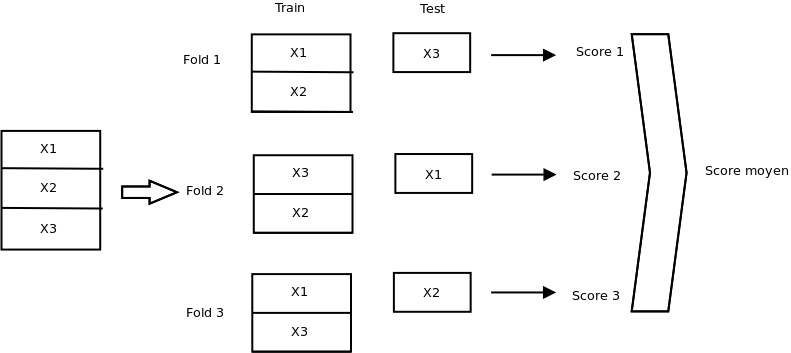
\includegraphics[scale = 0.25]{images/Valid_Croisee_param}
	\caption{Schéma de calcul d'un score par validation croisée}
	\label{fig:Valid_Croisee}
\end{figure}


Le principe de la validation croisée est de séparer un ensemble de données en plusieurs groupes de tailles équivalentes.
Sur le schéma de la  \autoref{fig:Valid_Croisee}, on peut observer un ensemble de données séparé en 3 avec $X_{1}$, $X_{2}$, $X_{3}$.
Chacun à tour de rôle sera utilisé pour l'apprentissage et le test. 
Sur les deux schémas, on peut lire \og{} score \fg{}, cela représente le résultat de la comparaison entre les prédictions et les vrais résultats par la régression linéaire. Ce score déterminera si notre prédiction est satisfaisante ou non. 

\begin{figure}[htpb]
	\centering
	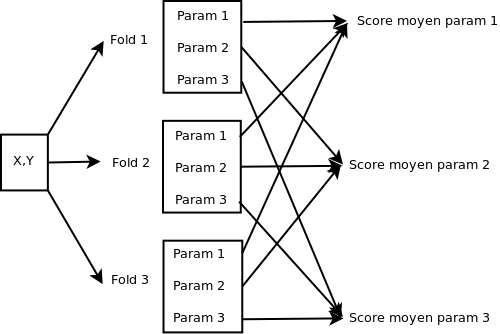
\includegraphics[scale = 0.25]{images/Valid_Croisee}
	\caption{Schéma de fonctionnement de la validation croisée}
	\label{fig:Valid_Croisee_param}
\end{figure}

Dans notre cas, les données seront divisées en 5 groupes qui tourneront à tour de rôle entre groupe d'apprentissage et groupe de test. 

Cette validation croisée est nécessaire dû à la faible quantité de sujets pour la recherche. Si nous avions 1000 sujets, cette méthode ne serait pas effectué mais pour obtenir un score assez précis pour être exploité, il nous faut cette validation croisée qui va nous donner un score de comparaison sur non pas sur 200 sujets mais sur 5 combinaisons possibles de ces 200 sujets. 

Toutes les méthodes décrites dans cette partie représentent énormément de temps de calcul.
Pour réduire ce temps, le module MapReduce va être utilisé. 